\documentclass{standalone}

\usepackage[dvipsnames]{xcolor}
\usepackage{tikz}
\usepackage{fontspec}

%\setmainfont[Scale=16]{nagayama_kai}
%\setmainfont[Scale=16]{kosugimaru}
\setmainfont[Scale=16]{epgyobld}
%\setmainfont[Scale=16]{epmgobld}

%\setmainfont[Scale=17.5]{ZinHenaBokuryu}
%\setmainfont[Scale=14]{NotoSerifJP-Black}
\begin{document}
\Huge

\begin{tikzpicture}
\node[opacity=0.3, inner sep=0pt, fill=white] at (0,0) {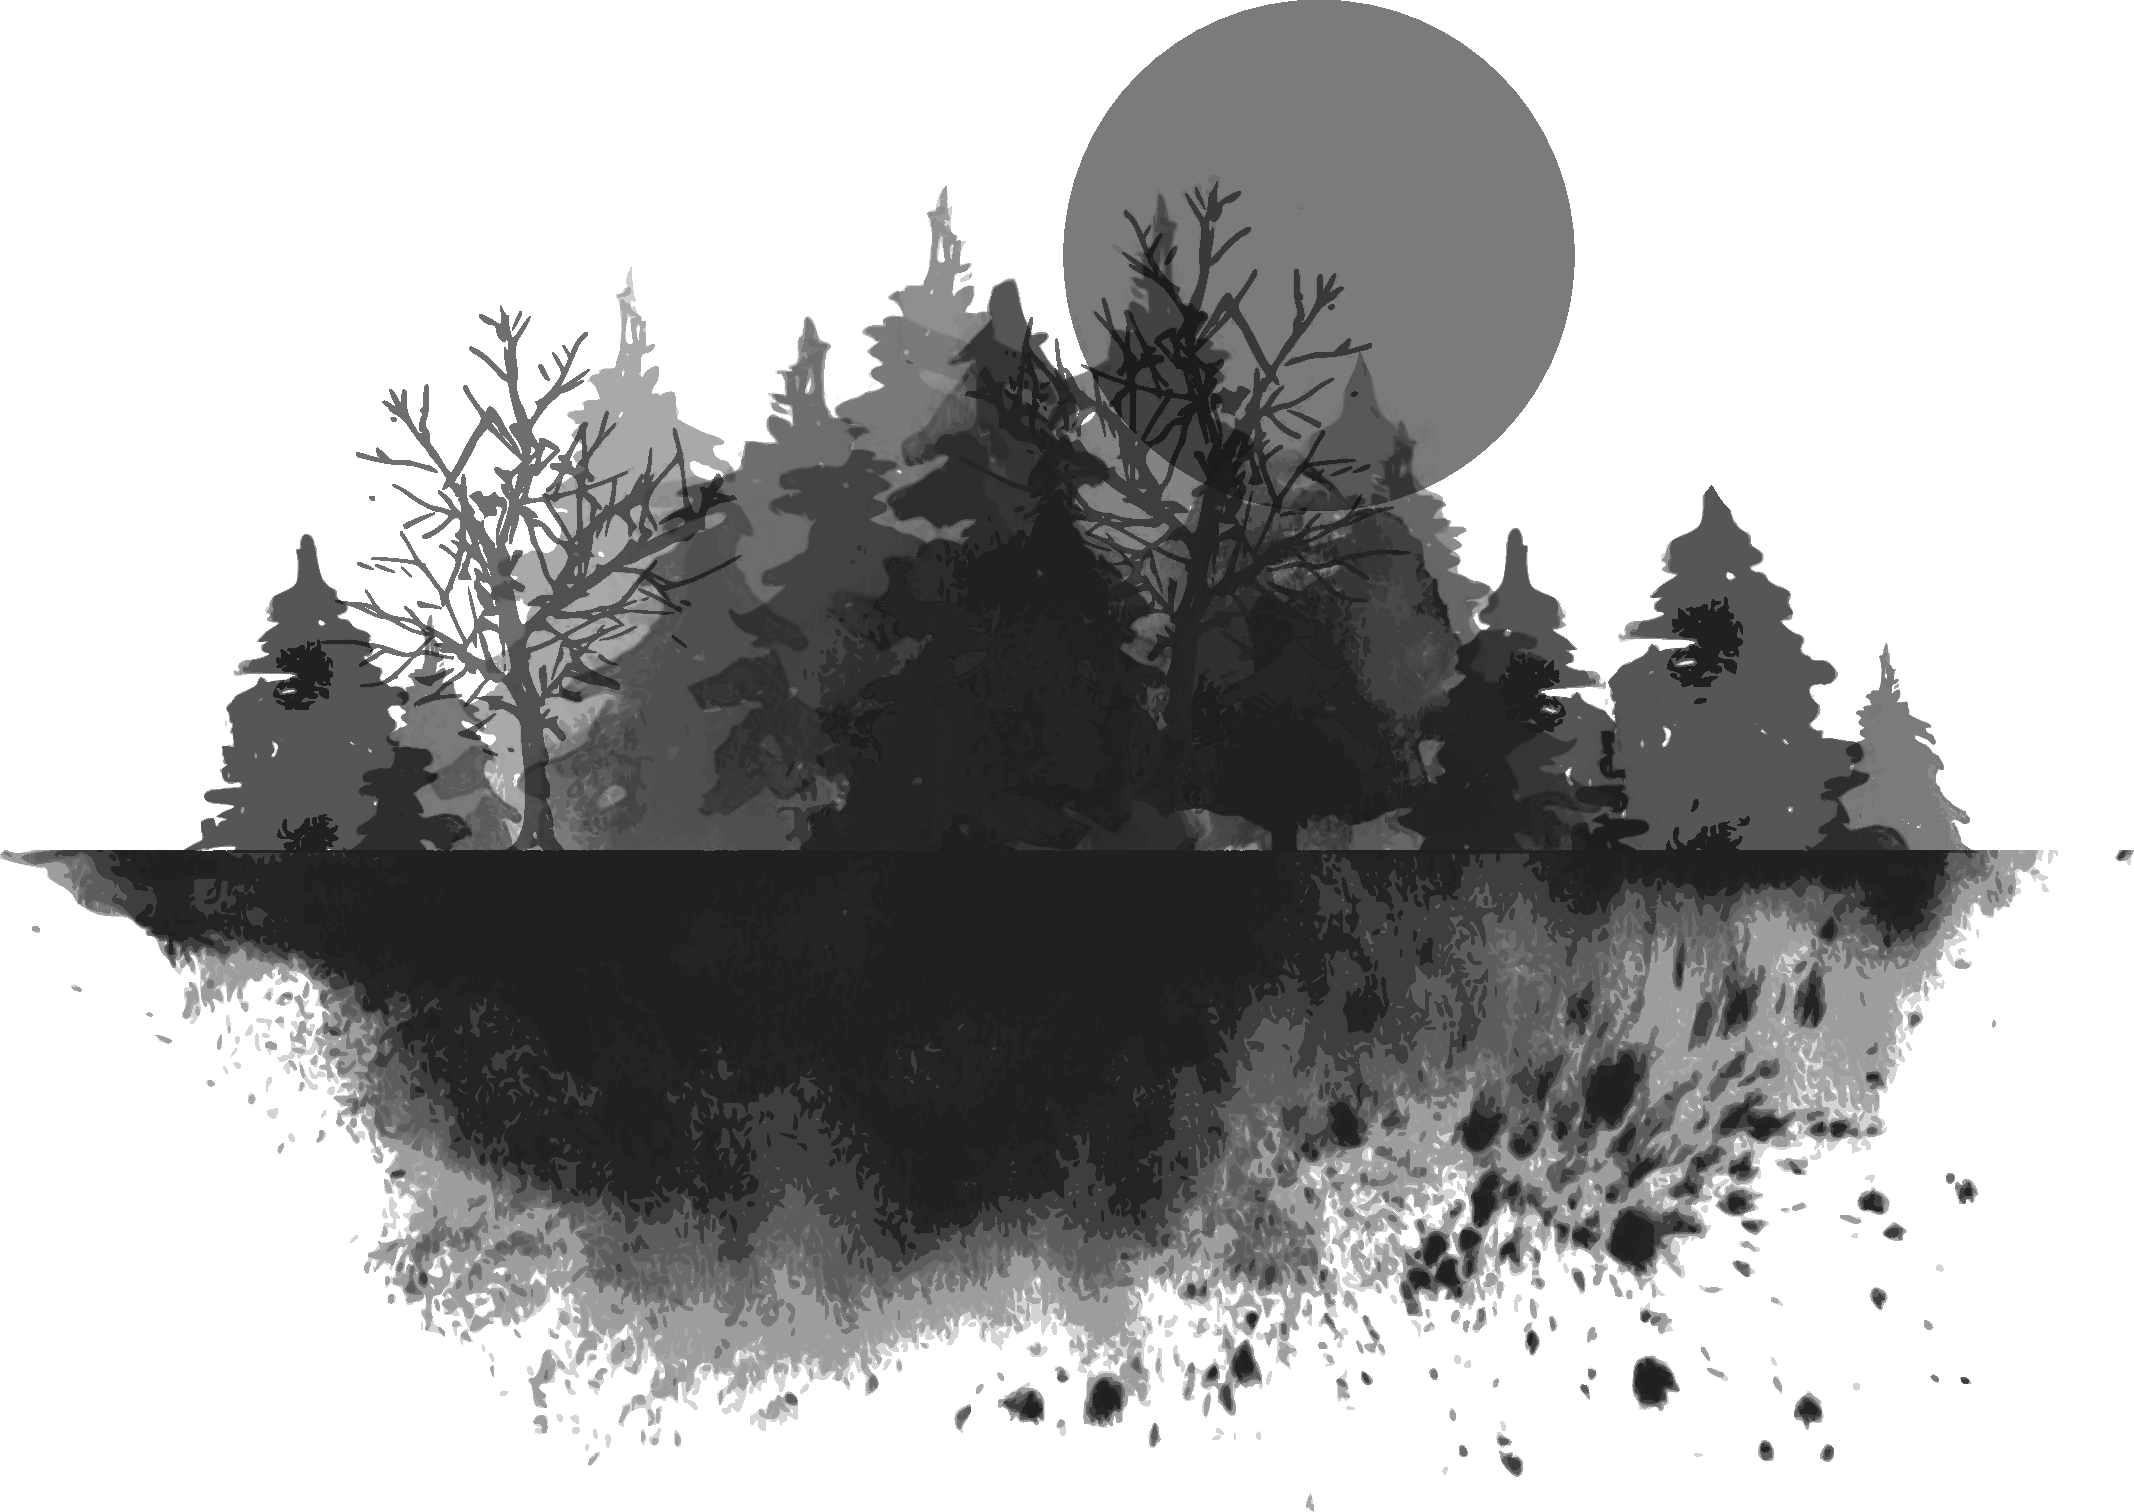
\includegraphics[width=19in]{landscape.png}};
%\node[text width=17.5in, align=center, inner sep=0pt] at (0,0in) {\textcolor{black}{The House of\\Waving Pines}};


\node[text width=17.5in, align=center, inner sep=0pt] at (0,0in) {\textcolor{Red}{演武線}};

%\node[text width=17.5in, align=center] at (0,5in) {\textcolor{black}{The House}};
%\node[text width=17.5in, align=center] at (0,0in) {\textcolor{black}{of}};
%\node[text width=17.5in, align=center] at (0,-3.5in) {\textcolor{black}{Waving Pines}};

\end{tikzpicture}

\end{document}